\documentclass[11pt]{memoir} % Maybe use Tufte ?
\usepackage{minitoc}
\usepackage[utf8]{inputenc}
\usepackage{amsmath,amsfonts,amssymb,wasysym}
\usepackage{media9, graphicx, wrapfig}
\usepackage{caption}
\usepackage{graphics,epsfig}
\usepackage{tabularx}	
\usepackage{subcaption}
\usepackage{mathrsfs}
\usepackage{listings}
\usepackage{multirow}

\usepackage[usenames, dvipsnames]{color, xcolor}
\usepackage{pgf}
\usepackage{appendix}
\usepackage{etoolbox}
\usepackage{booktabs}
\usepackage{gensymb}
\usepackage{verse}
\usepackage{adjustbox}
\usepackage{array}	 
\usepackage{todonotes}
\usepackage{marginnote}
\usepackage{lscape}
\usepackage{float}
\usepackage{marginfix}

\setcounter{minitocdepth}{2} 
\setlength{\mtcindent}{24pt} 
\renewcommand{\mtcfont}{\small} 
\renewcommand{\mtcSfont}{\small} 



\setcounter{tocdepth}{1} % Show sections
\setcounter{secnumdepth}{3} %Numbered sections
\setlength{\mtcindent}{0pt}




\setlength{\parindent}{3.5em}

\setlength{\parskip}{1.2em}


\newenvironment{rotatepage}%
{\clearpage\pagebreak[4]\global\pdfpageattr\expandafter{\the\pdfpageattr/Rotate 90}}%
{\clearpage\pagebreak[4]\global\pdfpageattr\expandafter{\the\pdfpageattr/Rotate 0}}%


\definecolor{codegreen}{rgb}{0,0.6,0}
\definecolor{codegray}{rgb}{0.5,0.5,0.5}
\definecolor{codepurple}{rgb}{0.58,0,0.82}
\definecolor{backcolour}{rgb}{0.95,0.95,0.92}

\lstdefinestyle{mystyle}{
	backgroundcolor=\color{backcolour},   
	commentstyle=\color{codegreen},
	keywordstyle=\color{magenta},
	numberstyle=\tiny\color{codegray},
	stringstyle=\color{codepurple},
	basicstyle=\ttfamily\footnotesize,
	breakatwhitespace=false,         
	breaklines=true,                 
	captionpos=b,                    
	keepspaces=true,                 
	numbers=left,                    
	numbersep=5pt,                  
	showspaces=false,                
	showstringspaces=false,
	showtabs=false,                  
	tabsize=2
}

\lstset{style=mystyle}
%\lstset{inputpath=../CodeForListings/}


\usepackage{tikz}
\usetikzlibrary{shapes.geometric, arrows}
\tikzstyle{startstop} = [rectangle, rounded corners, minimum width=3cm, minimum height=1cm,text centered, draw=black, fill=red!30]
\tikzstyle{io} = [trapezium, trapezium left angle=75, trapezium right angle=105, minimum width=1.5cm, minimum height=1cm, text centered, draw=black, fill=blue!30]
\tikzstyle{process} = [rectangle, minimum width=3cm, minimum height=1cm, text centered, draw=black, fill=orange!30]
\tikzstyle{decision} = [rectangle,, rounded corners, minimum width=2cm, minimum height=1cm, text centered, draw=black, fill=green!30]
\tikzstyle{arrow} = [thick,->,>=stealth]


\newcommand{\attrib}[1]{%
\nopagebreak{\raggedleft\footnotesize #1\par}}
\renewcommand{\poemtitlefont}{\normalfont\large\itshape\centering}


\captionsetup[subsub]{font=footnotesize,labelfont={bf,sf}}
\setsecnumdepth{subsubsection}
\settocdepth{subsubsection}



\BeforeBeginEnvironment{appendices}{\clearpage}

\usepackage{subfiles}
\graphicspath{{../Figures/}{../../Figures/}}



\dominitoc

\title{\textbf{Laki To Tambora} \\ A study of ice cores}
\author{Thea Quistgaard}
\date{Master Thesis 2020/2021}

\begin{document}

\lstset{language=python}
\frontmatter

%\maketitle





%\newpage



\poemtitle{Darkness}
\settowidth{\versewidth}{Rayless, and pathless, and the icy earth}
\begin{verse}[\versewidth]
	I had a dream, which was not all a dream.\\
	The bright sun was extinguish'd, and the stars\\
	Did wander darkling in the eternal space,\\
	Rayless, and pathless, and the icy earth\\
	Swung blind and blackening in the moonless air;\\
	Morn came and went—and came, and brought no day.
	\label{Verse:Darkness}
\end{verse}
\attrib{Lord Byron (1788--1824), July 1816}




\begin{figure}[h]
	\centering
	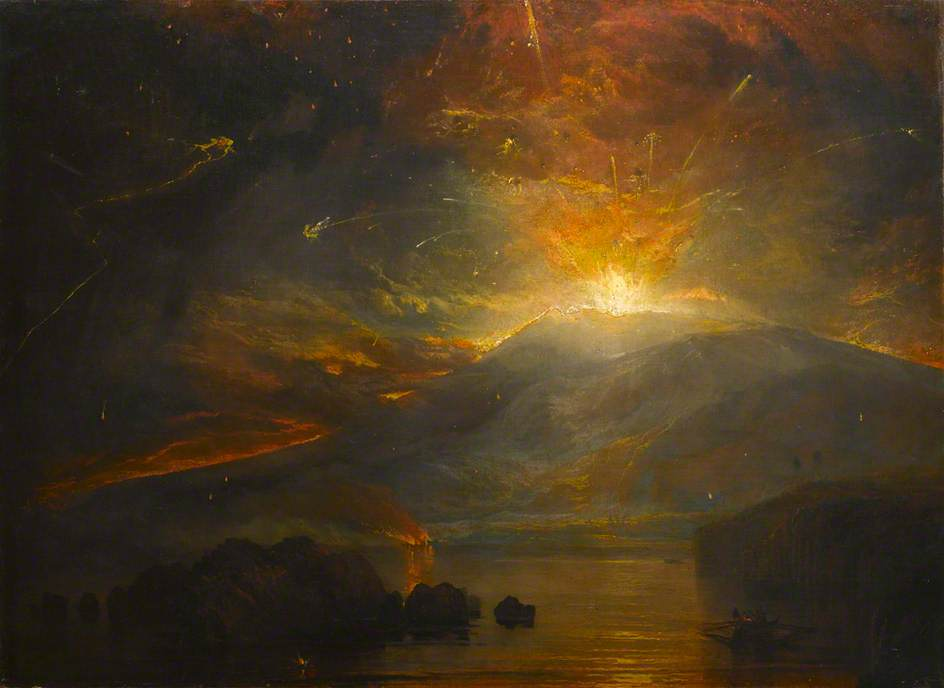
\includegraphics[width=0.8\textwidth]{TurnerEruptionofSoufriere-Mountains.jpg}
	\caption[\textit{The Eruption of the Soufriere Mountains}, Turner 1815]{J. M. W. Turner: \textit{The Eruption of the Soufriere Mountains in the Island of St Vincent, 30 April 1812}, 1815}
	\label{Fig:Turner}
\end{figure}

\newpage
\section*{Acknowledgments}
\label{Acknowledgments}
Firstly, I would like to thank my supervisors Vasileios Gkinis and James Avery for guidance and never ending ideas and inputs. It has been an honour to work with so inspiring people, across of two different fields. Though I have not had the capacity to implement all ideas debated and juggled, I appreciated all the shared knowledge and curiosity, so apparent in both of you. In addition, I send all my thanks and appreciation to all the wonderful people situated at PICE. Through lockdowns and dark winters, through laughter and sun on the terrace, it has been a pleasure to be surrounded with that many sweet, engaged and caring people. A special thanks to Meg Harlan, Mikkel Rasmus Schmidt, Rebekka Frøystad and all the other students at PICE for making it feel like home. I would also like to send my thanks to my loving family, Hans, Bodil and Daniel, who has - through my entire life - been the wind in my back and the first ones to pop open a bottle of champagne. I could not have done this without you. A warmhearted thanks to Marcel Løvendahl Jørgensen, you will always be in my heart, thank you for all the support in the last many years. Furthermore, I send my appreciation to all my wonderful friends, Signe, Sofie, Josephine, Nadia, Simon, Mikkel, and many many more. 
So many people have set their mark on my studies at the Niels Bohr Institute, both personally and professionally, and it is a time, I will always treasure. 

\newpage
\section*{Abstract}
\label{Abstract}
A difficulty when studying data from ice cores, is the processes of densification and diffusion throughout the firn column. These processes attenuates some of the signal of the measured data, i.e. the water isotopic ratios or the chemical compositions of the ice. This work focuses on restoring the most likely signal in a given depth section of an ice core, through a method referred to as 'back-diffusion'. This method attempts to restore a signal by back diffusing it with an estimated diffusion length, $\sigma$. This diffusion length is affected by a number of different parameters, especially interesting by the temperature at deposition. So to give a qualified estimate on the temperature at a given time, it is of utmost importance to estimate the diffusion length as accurate and precise as possible. The restoration is achieved through a number of different computational methods, with a specific focus on a constrained optimization routine. This routine assumes a number of constraint over the depth series, especially the number of years expected in the section. This dating is made through Electrical Conductivity Measurements, where the two historically well documented volcanic eruptions of Laki (1783) and Tambora (1815) are visible. The method is tested on five different ice cores, from the Alphabet ice core series, all shallow cores drilled in the vicinity of the Crête ice core.
The method has room for improvement, especially some of the simpler assumptions like the constraints and the optimization routine could benefit from further development. Moreover, the work carried out in this thesis leaves room for additional examination and development, but lays a good foundation to be used as a stepping stone in future research.
\newpage

%\listoftodos

\tableofcontents \mtcaddchapter




\newpage

\listoffigures \mtcaddchapter

\listoftables \mtcaddchapter 



\mainmatter
	



\chapter[Introduction][Introduction]{Introduction}
\label{Chap:Intro}
\subfile{../Chapters/Introduction/Chapter_Introduction2}


\chapter[Ice Theory][Ice Theory]{The Theory of Ice Cores}
\label{Chap:IceTheory}

\subfile{../Chapters/IceTheory/Chapter_IceTheory2}


\chapter[Data][Data]{Isotopic Data: Laki to Tambora as Seen in Five Ice Cores.}
\label{Chap:Data}

\subfile{../Chapters/Data/Chapter_Data2}



\chapter[Signal Analysis \& Comp. Meth.][Signal Analysis \& Comp. Meth.]{Signal Analysis and Computational Methods}
\label{Chap:SigAnalCompMeth}
\subfile{../Chapters/SignalAnalysis/Chapter_SignalAnalysisAndCompMeth}


%\chapter[Computational Methods]{Computational Methods}

%\subfile{../Chapters/ComputationalMethods/Chapter_ComputationalMethods2}


\chapter[Method and Discussion][Method and Discussion]{Estimating $\sigma$ from Data: Methods, Algorithms and Discussion}
\label{Chap:MethodAndDiscussion}
\subfile{../Chapters/Method/Chapter_Method2}


\chapter[Results]{Results}
\subfile{../Chapters/Results/Chapter_Results2}
\label{Chap:Results}

%\chapter[Temperature Reconstruction]{Temperature Reconstruction}
´
%\subfile{../Chapters/TemperatureReconstruction/Chapter_TemperatureReconstruction2}


%\chapter[Layer Counting][Layer Counting]{Layer Counting and Annual Layer Thickness Estimation}

%\subfile{../Chapters/LayerCounting/Chapter_LayerCounting2}



\chapter[Conclusion and Outlook][Conclusion and Outlook]{Conclusion and Outlook}
\label{Chap:ConclusionAndOutlook}
\subfile{../Chapters/Conclusion/Chapter_Conclusion2}


\backmatter

\bibliographystyle{plain} 
\bibliography{/home/thea/Documents/Bibliographies/MasterThesis.bib}

%https://reader.elsevier.com/reader/sd/pii/S0039914019305375?token=2655091B0658E162E9C8C95D1AB1B21B2289F565CA3596158B63639417D66BEFC3345B6AD8E27A8453C968554CEDE2CB

%https://pubs.acs.org/doi/pdf/10.1021/acs.analchem.9b04811
\appendix 
\addcontentsline{toc}{chapter}{APPENDICES}

\chapter[Appendices][Appendices]{Appendices}
\subfile{../Chapters/Appendix/Chapter_Appendix2}
	
\end{document}